\documentclass[portrait, a1paper, fontscale=.5]{baposter}

\begin{document}
    
\newcommand{\lo}{\left(}
\newcommand{\ro}{\right)} 
\newcommand{\bs}[1]{\textit{\textbf{#1}}}
\newcommand{\bsm}[1]{\boldsymbol{#1}}
\newcommand{\pds}[2]{\frac{\partial{#1}}{\partial{#2}}}
\newcommand{\pdv}[2]{\frac{\partial{#1}}{\partial{\bs{#2}}}}
\renewcommand{\d}[2]{\frac{d{#1}}{d{#2}}}
\newcommand{\mc}[1]{\mathcal{#1}}
\newcommand{\phib}{\bsm{\varphi}}
\newcommand{\esssup}{\operatornamewithlimits{ess\,sup}}

\newenvironment{proof}[1][Proof]{\begin{trivlist}
\item[\hskip \labelsep {\bfseries #1}]}{\end{trivlist}}


\def\be{\begin{equation}}
\def\ee{\end{equation}}
\def\bfig{\begin{figure}}
\def\efig{\end{figure}}
\def\bd{\begin{displaymath}}
\def\ed{\end{displaymath}}
\def\ba{\begin{array}}
\def\ea{\end{array}}

\newcommand{\bfa}{\mbox{\boldmath $a$}}
\newcommand{\bfb}{\mbox{\boldmath $b$}}
\newcommand{\bfc}{\mbox{\boldmath $c$}}
\newcommand{\bfd}{\mbox{\boldmath $d$}}
\newcommand{\bfe}{\mbox{\boldmath $e$}}
\newcommand{\bff}{\mbox{\boldmath $f$}}
\newcommand{\bfg}{\mbox{\boldmath $g$}}
\newcommand{\bfh}{\mbox{\boldmath $h$}}
\newcommand{\bfi}{\mbox{\boldmath $i$}}
\newcommand{\bfj}{\mbox{\boldmath $j$}}
\newcommand{\bfk}{\mbox{\boldmath $k$}}
\newcommand{\bfl}{\mbox{\boldmath $l$}}
\newcommand{\bfm}{\mbox{\boldmath $m$}}
\newcommand{\bfn}{\mbox{\boldmath $n$}}
\newcommand{\bfo}{\mbox{\boldmath $o$}}
\newcommand{\bfp}{\mbox{\boldmath $p$}}
\newcommand{\bfq}{\mbox{\boldmath $q$}}
\newcommand{\bfr}{\mbox{\boldmath $r$}}
\newcommand{\bfs}{\mbox{\boldmath $s$}}
\newcommand{\bft}{\mbox{\boldmath $t$}}
\newcommand{\bfu}{\mbox{\boldmath $u$}}
\newcommand{\bfuhp}{\mbox{{\boldmath $u$}$_{h, p}$}}
\newcommand{\bfv}{\mbox{\boldmath $v$}}
\newcommand{\bfvhp}{\mbox{{\boldmath $v$}$_{h, p}$}}
\newcommand{\bfw}{\mbox{\boldmath $w$}}
\newcommand{\bfx}{\mbox{\boldmath $x$}}
\newcommand{\bfy}{\mbox{\boldmath $y$}}
\newcommand{\bfz}{\mbox{\boldmath $z$}}
%
\newcommand{\bfA}{\mbox{\boldmath $A$}}
\newcommand{\bfB}{\mbox{\boldmath $B$}}
\newcommand{\bfC}{\mbox{\boldmath $C$}}
\newcommand{\bfD}{\mbox{\boldmath $D$}}
\newcommand{\bfE}{\mbox{\boldmath $E$}}
\newcommand{\bfF}{\mbox{\boldmath $F$}}
\newcommand{\bfG}{\mbox{\boldmath $G$}}
\newcommand{\bfH}{\mbox{\boldmath $H$}}
\newcommand{\bfI}{\mbox{\boldmath $I$}}
\newcommand{\bfJ}{\mbox{\boldmath $J$}}
\newcommand{\bfK}{\mbox{\boldmath $K$}}
\newcommand{\bfL}{\mbox{\boldmath $L$}}
\newcommand{\bfM}{\mbox{\boldmath $M$}}
\newcommand{\bfN}{\mbox{\boldmath $N$}}
\newcommand{\bfO}{\mbox{\boldmath $O$}}
\newcommand{\bfP}{\mbox{\boldmath $P$}}
\newcommand{\bfQ}{\mbox{\boldmath $Q$}}
\newcommand{\bfR}{\mbox{\boldmath $R$}}
\newcommand{\bfS}{\mbox{\boldmath $S$}}
\newcommand{\bfT}{\mbox{\boldmath $T$}}
\newcommand{\bfU}{\mbox{\boldmath $U$}}
\newcommand{\bfV}{\mbox{\boldmath $V$}}
\newcommand{\bfW}{\mbox{\boldmath $W$}}
\newcommand{\bfX}{\mbox{\boldmath $X$}}
\newcommand{\bfY}{\mbox{\boldmath $Y$}}
\newcommand{\bfZ}{\mbox{\boldmath $Z$}}
\newcommand{\bfone}{\mbox{\boldmath $1$}}
%
\def\Hcurl{{\bfH({\rm curl})}}
\def\Hdiv{{\bfH({\rm div})}}
%\def\R{{\rm I\hspace{-0.9mm}R}}
\def\R{\boldmath R}
\def\C{\boldmath C}
\def\Q{\boldmath Q}

%
\def\calB{{\cal B}}
\def\calF{{\cal F}}
\def\calM{{\cal M}}
\def\calS{{\cal S}}
\def\calA{{\cal A}}
\def\calG{{\cal G}}
\def\calE{{\cal E}}
%\def\cale{{\cal e}}
\def\calL{{\cal L}}
\def\calD{{\cal D}}
\def\calI{{\cal I}}
\def\calJ{{\cal J}}
\def\calT{{\cal T}}
\def\calY{{\cal Y}}
\def\calZ{{\cal Z}}
%
\newcommand{\ds}{\displaystyle}
%
\newcommand{\bfalp}{\mbox{\boldmath $\alpha$}}
\newcommand{\bfbet}{\mbox{\boldmath $\beta$}}
\newcommand{\bfgam}{\mbox{\boldmath $\gamma$}}
\newcommand{\bfdel}{\mbox{\boldmath $\delta$}}
\newcommand{\bfeps}{\mbox{\boldmath $\epsilon$}}
\newcommand{\bfvareps}{\mbox{\boldmath $\varepsilon$}}
\newcommand{\bfzet}{\mbox{\boldmath $\zeta$}}
\newcommand{\bfeta}{\mbox{\boldmath $\eta$}}
\newcommand{\bfthet}{\mbox{\boldmath $\theta$}}
\newcommand{\bfiot}{\mbox{\boldmath $\iota$}}
\newcommand{\bfkap}{\mbox{\boldmath $\kappa$}}
\newcommand{\bflam}{\mbox{\boldmath $\lambda$}}
\newcommand{\bfmu}{\mbox{\boldmath $\mu$}}
\newcommand{\bfnu}{\mbox{\boldmath $\nu$}}
\newcommand{\bfxi}{\mbox{\boldmath $\xi$}}
\newcommand{\bfomega}{\mbox{\boldmath $\omega$}}
\newcommand{\bfzeta}{\mbox{\boldmath $\zeta$}}
\newcommand{\bfpi}{\mbox{\boldmath $\pi$}}
\newcommand{\bfrho}{\mbox{\boldmath $\rho$}}
\newcommand{\bfsig}{\mbox{\boldmath $\sigma$}}
\newcommand{\bftau}{\mbox{\boldmath $\tau$}}
\newcommand{\bfups}{\mbox{\boldmath $\upsilon$}}
\newcommand{\bfphi}{\mbox{\boldmath $\phi$}}
\newcommand{\bfvarphi}{\mbox{\boldmath $\varphi$}}
\newcommand{\bfchi}{\mbox{\boldmath $\chi$}}
\newcommand{\bfpsi}{\mbox{\boldmath $\psi$}}
\newcommand{\bfome}{\mbox{\boldmath $\omega$}}
%
\newcommand{\bfGam}{\mbox{\boldmath $\Gamma$}}
\newcommand{\bfDel}{\mbox{\boldmath $\Delta$}}
\newcommand{\bfThet}{\mbox{\boldmath $\Theta$}}
\newcommand{\bfLam}{\mbox{\boldmath $\Lambda$}}
\newcommand{\bfXi}{\mbox{\boldmath $\Xi$}}
\newcommand{\bfPi}{\mbox{\boldmath $\Pi$}}
\newcommand{\bfSig}{\mbox{\boldmath $\Sigma$}}
\newcommand{\bfUps}{\mbox{\boldmath $\Upsilon$}}
\newcommand{\bfPhi}{\mbox{\boldmath $\Phi$}}
\newcommand{\bfPsi}{\mbox{\boldmath $\Psi$}}
\newcommand{\bfOme}{\mbox{\boldmath $\Omega$}}

\newcommand{\ptl}{{\partial}}
\newcommand{\nab}{{\nabla}}

\newcommand{\Tau}{{\cal{T}}}

\def \span {{\rm span}}

\newcommand\dS{\mbox{d\boldmath$S$}}
\renewcommand\O{{\cal O}}
\renewcommand\P{{\cal P}}
\renewcommand\H{{\cal H}}

\newcommand{\bfptl}{\mbox{\boldmath $\partial$}}
\newcommand{\bfell}{\mbox{\boldmath $\ell$}}
\newcommand{\bfnab}{\mbox{\boldmath $\nabla$}}
\newcommand{\bfinfty}{\mbox{\boldmath $\infty$}}
\newcommand{\bfto}{\mbox{\boldmath $\to$}}
\newcommand{\doubleIR}{\mbox{$I \!\!\!\! R$}}
\newcommand{\doubleIC}{\mbox{$I \!\!\! C$}}
\newcommand{\dlbracket}{\mbox{$[ \! |$}}
\newcommand{\drbracket}{\mbox{$] \! |$}}
\newcommand{\dlx}{\mbox{$x \!\!\!\! x$}}
\newcommand{\notO}{\mbox{$O \!\!\!\! /$}}
\newcommand{\tm}{\mbox{$^{TM}$}}

\newcommand{\dd}{\mathrm d}
\newcommand{\der}[2]{\frac{{\dd} #1}{{\dd} #2}}
\newcommand{\pard}[2]{\frac{\partial #1}{\partial #2}}
\newcommand{\pardx}[3]{\frac{\partial^{#1} #2}{\partial #3^{#1}}}
\newcommand{\vct}[1]{\boldsymbol{#1}}
\newcommand{\op}[1]{{\cal{#1}}}
\newcommand{\lp}{\left(}
\newcommand{\rp}{\right)}
\newcommand{\lb}{\left[}
\newcommand{\rb}{\right]}
\newcommand{\lsp}{\left\langle}
\newcommand{\rsp}{\right\rangle}
\newcommand{\lcb}{\left\lbrace}
\newcommand{\rcb}{\right\rbrace}
\newcommand{\li}{\left.}
\newcommand{\ri}{\right.}
\newcommand{\tens}[1]{\mbox{\boldmath$#1$}}

\newcommand{\mrx}{\mathrm{\mathbf{x}}}
\newcommand{\mrJ}{\mathrm{\mathbf{J}}}
\newcommand{\mrR}{\mathrm{\mathbf{R}}}
\newcommand{\mrH}{\mathrm{\mathbf{H}}}
\newcommand{\mrF}{\mathrm{\mathbf{F}}}
\newcommand{\mrS}{\mathrm{\mathbf{S}}}
\newcommand{\mrFi}{\mathrm{\mathbf{F}}_i}
\newcommand{\mrv}{\mathrm{\mathbf{v}}}
\newcommand{\mrvh}{\mathrm{\mathbf{v}}_h}
\newcommand{\mrvhl}{\mathrm{\mathbf{v}}_{hl}}
\newcommand{\mrvhi}{\mathrm{\mathbf{v}}_{hi}}
\newcommand{\mrvhm}{\mathrm{\mathbf{v}}_{hm}}
\newcommand{\mrw}{\mathrm{\mathbf{w}}}
\newcommand{\mrPsi}{\mathrm{\mathbf{\Psi}}}
\newcommand{\mrPsii}{\mathrm{\mathbf{\Psi_i}}}
\newcommand{\mrA}{\mathrm{\mathbf{A}}}
\newcommand{\mrAi}{\mathrm{\mathbf{A}}_i}

\begin{poster}{
	grid=false,
	columns=6,
	borderColor=bordercolor,
	headerColorOne=headercolorone,
	headerFontColor=headerfontcolor,
	headershape=rectangle,
	headershade=plain,
	headerborder=closed,
	boxColorOne=boxcolorone,
	textborder=rectangle,
	background=plain,
	boxshade=plain
}

\background{
\begin{tikzpicture}[remember picture, overlay]%
	\draw (current page.north west) node[anchor=north west] 
{
\includegraphics[width=1.0\paperwidth,height=1.0\paperheight]{rice-background}};
\end{tikzpicture}

{\postertitle{Distributed Implicit Discontinuous Galerkin MHD Solver}}
{\posterauthors{Lukas Korous, Jan Skala, Jan Kotek, Pavel Karban}{University of West Bohemia - Faculty of Electrical Engineering, Czech Republic\\ 
Regional Innovation Centre for Electrical Engineering, Department of Theory of Electrical Engineering\\
Astronomical Institute of Czech Academy of Sciences, Ondřejov, Czech Republic\\
E-mail: korous@kte.zcu.cz, jan.skala@asu.cas.cz, jankotek@email.cz, karban@kte.zcu.cz}} }

%{
\includegraphics{fel}}
%{\includegraphics{kte}}

\headerbox{\textbf{Abstract}}{name=1,column=0,row=0,span=2}{
The work aims at solving the nonlinear ideal MHD equations using the Discontinuous Galerkin (DG) method. The nonlinear equations will be solved implicitly, and the problem of differentiating non-differentiable numerical fluxes (such as HLLD), will be taken care of by constructing the jacobian using numerical differentiation from the residual and using damped Newton's method. Overshoots and undershoots present in the vicinity of physical shock waves will be accounted for adopting a post-processing step implementing the vertex-based limiter.
\ \\
\ \\
This work is being implemented using the FE libraries deal.II and Trilinos in 3D and fully parallel/distributed manner, and once finished will be available at a public software repository.
\ \\
\ \\
There are several phenomena in the universe that we can look at as magnetohydrodynamic in nature - planets consisting of metals, interplanetary space, stars. As for the stars, these phenomena include spots, solar flares, solar winds, space weather. To study these phenomena, it is important that we are able to model them at a reasonable scale, in a reasonable detail, but most importantly - model them in a physically correct way. This means that on the path from our physical / mathematical model to numerical solutions, our algorithms should not spoil the solution by introducing non-physical oscillations, be in conflict with the model (having $\mathrm{div}\,\mathbf{B}=0$), add artificial diffusion, etc.

}

\headerbox{\textbf{Formulation of the Problem}}{name=2,column=0,row=0,span=2,below=1}{
Ideal MHD equations in the conservative form read:
\be
\label{conservativeGeneric} \pds{\mrPsi}{t} + \nabla \cdot \mrF\lo\mrPsi\ro = \mrS,
\ee
where $\mrPsi$ is the \textit{state vector}, $\mrF_i,\ i = 1, 2, 3$ are the \textit{fluxes}, and $\mrS$ is the \textit{source term}:

\begin{eqnarray}
\mrPsi \hspace{-3mm}  & = & \hspace{-3mm}  \lo\rho, \pi_1, \pi_2, \pi_3, U, B_1, B_2, B_3\ro,
\\
\mrF_i \hspace{-3mm} & = & \hspace{-3mm} \lo\begin{array}{c}
    \hspace{-3mm} \pi_i \\
    \hspace{-3mm} \frac{\pi_1 \pi_i}{\rho} - B_1 B_i + \frac12 \delta_{1i} \lo p + U_m\ro \\
    \hspace{-3mm} \frac{\pi_2 \pi_i}{\rho} - B_1 B_i + \frac12 \delta_{2i} \lo p + U_m\ro \\
    \hspace{-3mm} \frac{\pi_3 \pi_i}{\rho} - B_1 B_i + \frac12 \delta_{3i} \lo p + U_m\ro \\
    \hspace{-3mm} \frac{\pi_i}{\rho} \lo \frac{\gamma}{\gamma - 1} p + U_k\ro + \frac{2}{\rho} \varepsilon_{ijk} \lo \pi_k B_i - \pi_i B_k\ro B_k  \\
    \hspace{-3mm} \frac{\pi_i B_1 - \pi_1 B_i}{\rho} \\
    \hspace{-3mm} \frac{\pi_i B_2 - \pi_2 B_i}{\rho} \\
    \hspace{-3mm} \frac{\pi_i B_3 - \pi_3 B_i}{\rho}\\
\end{array}\ro,
\\
\mrS \hspace{-3mm}  & = & \hspace{-3mm}  \lo0, \rho g_1, \rho g_2, \rho g_3, \bfpi \cdot \bfg, 0, 0, 0\ro.
\end{eqnarray}
Here, $\rho$ is the plasma density, $\pi_1, \pi_2, \pi_3$ are the $x-, y-,$ and $z-$ momentum components respectively. $U$ is the total energy, $B_1, B_2, B_3$ are the three components of magnetic field. Remaining quantities are $p$ - plasma pressure, $U_k$ - kinetic energy, $U_m$ - magnetic energy, and $\bfg$ gravitational acceleration with components $g_1, g_2, g_3$.
}

\headerbox{\textbf{DG Formulation}}{name=3,column=2,row=0,span=2}{
DG formulation of the resulting space-discretized problem reads
\begin{eqnarray}
\label{DG2} \int_{\Omega_{t}} \pds{{\mrPsi_h}}{t} \mrvh
    & - & \sum_{K_i \in T_h}\int_{K_i}\mrF\lo{\mrPsi_h}\ro \lo\nabla \cdot \mrvh\ro\\
    \nonumber & + & \sum_{\Gamma_{ij}\in\Gamma_I} \int_{\Gamma_{ij}} \mrH\lo{\mrPsi_h}|_{ij}, {\mrPsi_h}|_{ji}, \bfn_{ij}\ro \mrvh\\
    \nonumber & + & \sum_{\Gamma_{i}\in\Gamma_B} \int_{\Gamma_{i}} \mrH\lo{\mrPsi_h}|_{i}, \overline{{\mrPsi_h}|_{i}}, \bfn_{i}\ro \mrvh\\
    \nonumber & = & \int_{\Omega_{t}} \mrS \mrvh,
\end{eqnarray}
where $\mrvh$ is a test function, $\Gamma_I$ is a set of all internal interfaces in the mesh, and $\Gamma_{ij}\in\Gamma_I$ an interface between two elements - $K_i$ and $K_j$. Similarly $\Gamma_B$ is a set of all boundary interfaces in the mesh, and $\Gamma_{i}\in\Gamma_B$ an interface on the boundary that neighbors the element $K_i$. Meaning of $\overline{{\mrPsi_h}|_{i}}$ depends on the boundary conditions.

$\mrH\lo{\mrPsi_h}|_{ij}, {\mrPsi_h}|_{ji}, \bfn_{ij}\ro$ is the \textit{numerical flux} between states ${\mrPsi_h}|_{ij}$ and ${\mrPsi_h}|_{ji}$ in the direction of $\bfn_{ij}$.

%Deriving the fully (space- and time-) discretized problem using Crank-Nicolson scheme is straightforward.
}

\headerbox{\textbf{Solving the nonlinear problem}}{name=4,column=2,row=0,span=2,below=3}{
We would like to use the Newton's method to solve the nonlinear problem arising from discretizing (\ref{DG2}) in time using Crank-Nicolson scheme. Damped Newton's method (with damping factor $\alpha$) performs iterations
\begin{eqnarray}
\label{Newton}
\mrJ\lo\mrx^{n}_{k+1}\ro\lo\Delta\mrx^{n}_{k+1}\ro & = & -\mrR\lo\mrx^{n}_{k+1}\ro\\
\nonumber
\mrx^{n+1}_{k+1} & = & \mrx^{n}_{k+1} + \alpha\Delta\mrx^{n}_{k+1},
\end{eqnarray}
for $n = 0, ...$, where $\mrR\lo\mrx^{n}_{k+1}\ro$ is the \textit{residual}, $\mrJ\lo\mrx^{n}_{k+1}\ro = \frac{\mathrm{d}\mrR\lo\mrx^{n}_{k+1}\ro}{\mathrm{d}\mrx^{n}_{k+1}}$ the \textit{jacobian}, $\mrx^{0}_{k+1} = \mrx_{k}$ and $\mrx_{k}$ is the DG solution vector from the $k$-th time step. For the residual, we have
\begin{eqnarray}
\mrR\lo\mrx\ro_i & = & \int_{\Omega_{t}} \frac{\mrPsi_h}{\Delta t} + \sum_{K_i \in T_h}\int_{K_i}\mrF\lo{\mrPsi_h}\ro \lo\nabla \cdot \mrvhi\ro\\
\nonumber & - & \sum_{\Gamma_{ij}\in\Gamma_I} \int_{\Gamma_{ij}} \mrH\lo{\mrPsi_h}|_{ij}, {\mrPsi_h}|_{ji}, \bfn_{ij}\ro \mrvhi\\
\nonumber & - & \sum_{\Gamma_{i}\in\Gamma_B} \int_{\Gamma_{i}} \mrH\lo{\mrPsi_h}|_{i}, \overline{{\mrPsi_h}|_{i}}, \bfn_{i}\ro \mrvhi + \int_{\Omega_{t}} \mrS \mrvhi,
\end{eqnarray}
where $\mrvhi$ is the $i$-th test function, and $\mrPsi_h$ is the (global) function corresponding to $\mrx$.

The jacobian $\mrJ\lo\mrx^{n}_{k+1}\ro = \frac{\mathrm{d}\mrR\lo\mrx^{n}_{k+1}\ro}{\mathrm{d}\mrx^{n}_{k+1}}$ is calculated numerically (numerical differentiation implementation from Trilinos package Sacado is used).

The iterations in (\ref{Newton}) are performed until $||\mrR\lo\mrx^{n}_{k+1}\ro||$ is lower than a prescribed threshold. 
}

\headerbox{\textbf{Handling nonzero divergence}}{name=5a,column=2,row=0,span=2,below=4}{
An infamous problem in numerically solving the MHD equations, which is present regardless of the presence of the continuity of the sought solution, is satisfying \textit{Gauss's law}, i.e. the relationship
\be
\label{zeroDivergence}
\mathrm{div}\,\mathbf{B}=0,
\ee
to tackle this, an exactly divergence free FE space is a mathematically clean and fully reliable method how to satisfy the relation \ref{zeroDivergence}, as opposed to methods of \textit{divergence cleaning}, or \textit{Constrained-Transport (CT)}. In order to create a generic solver, it is a very favorable method.
}

\headerbox{\textbf{Attributes of DG solution}}{name=5,column=4,row=0,span=2}{
There are several topics to be dealt with when solving MHD equations numerically using the DG method.
First one is the selection of numerical flux $\mrH\lo{\mrPsi_h}|_{ij}, {\mrPsi_h}|_{ji}, \bfn_{ij}\ro$ that should be as little diffusive as possible, and should satisfy the relations $\mrH\lo{\mrPsi_h}, {\mrPsi_h}, \bfn\ro = \mrF\lo{\mrPsi_h}\ro \cdot \bfn$ and $\mrH\lo{\mrPsi_1}, {\mrPsi_2}, \bfn\ro = \mrH\lo{\mrPsi_2}, {\mrPsi_1}, -\bfn\ro$. For the ideal MHD we chose the HLLD flux.
\ \\
\ \\
Another aspect of the solution, which occurs both in continuous and discontinuous FE simulations of the MHD system are spurious (nonphysical) oscillations appearing in the solution near discontinuities or sharp fronts. Here, in DG, the problem is much smaller than in the continuous case, as the instabilities occur only in regions adjacent to the sharp fronts.
\ \\
\ \\
Our goal is to build a software package that should give a reasonable and physically correct solution to all sorts of problems, a suitable method to handle discontinuities must not change the physics (as is the case in e.g. artificial diffusion) and must not require fine-tuning parameters for it to work. Therefore we chose a parameter-less method of post-processing nature (which does not change the equations being solved). Such a method is the \textit{Vertex-based limiter} developed by D. Kuzmin, and successfully applied to DG for advection-diffusion problems in existing work.
}


\headerbox{\textbf{Numerical example}}{name=6,column=4,row=0,span=2,below=5}{
We present results from one benchmark - MHD Blast - designed at \itshape{www.astro.princeton.edu/~jstone/Athena/tests/blast/blast.html}.

The figures below are performed with a standard set of basis functions for DG - i.e. not with the exactly divergence free basis we want to use - that is a work-in-progress currently and it shall only stabilize and qualitatively improve the results.

The following figures show the density, magnitude of momentum, magnitude of magnetic field, and the pressure in the region $-0.5 \leq x \leq 0.5; -0.5 \leq y \leq 0.5$.\ \\
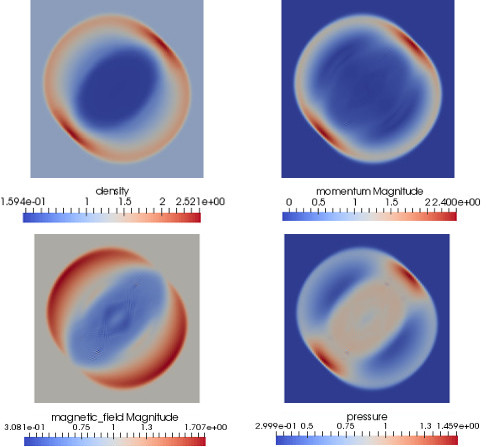
\includegraphics[width=0.98\columnwidth]{blastRes.jpg}
\captionof{figure}{MHD Blast benchmark results}
}

\headerbox{\textbf{Conclusion}}{name=7,column=4,row=0,span=2,below=6}{
The work is in progress, but already it is observable that the DG approach yields qualitatively good results, and due to the implementation of nonlinear solver, and parallel abilities of the used library deal.ii, the code is very efficient. Currently implemented feature is the mentioned vertex based limiter.
}

\headerbox{\textbf{Acknowledgment}}{name=9,column=4,row=0,span=2,below=7}{
This research has been supported by the Ministry of Education, Youth and Sports of the Czech Republic under the RICE – New Technologies and Concepts for Smart Industrial Systems, project No. LO1607.
\vspace{0.04cm}
}

\end{poster}

\end{document}